\documentclass{ctexbeamer}
\usepackage[backend = biber, style = gb7714-2015, url=false,gbtitlelink=true]{biblatex}
\addbibresource{ref.bib}
\usepackage{xeCJK}
\usepackage{graphicx}
\usepackage{grffile}
\usepackage{longtable}
\usepackage{wrapfig}
\usepackage{rotating}
\usepackage[normalem]{ulem}
\usepackage{amsmath}
\usepackage{textcomp}
\usepackage{amssymb}
\usepackage{capt-of}
\usepackage{minted}
\usepackage{hyperref}
\usetheme{CambridgeUS}
\author{董晨阳}
\date{\today}
\title{机器学习在企业风险管理中的应用举例}
\setbeamertemplate{bibliography item}{}
\setbeamertemplate{bibliography entry article}{}
\setbeamertemplate{bibliography entry title}{}
\setbeamertemplate{bibliography entry location}{}
\setbeamertemplate{bibliography entry note}{}
\begin{document}

\AtBeginSection[]
{
    \small\begin{frame}
        \frametitle{目录}
        \tableofcontents[
            sectionstyle=show/shaded,
            subsectionstyle=show/show/hide,
            subsubsectionstyle=show/show/show/hide
        ]
    \end{frame}
}
\maketitle
\begin{frame}
    \frametitle{目录}
    \tableofcontents[hideallsubsections]
    \small 笔记见 \url{https://ernestdong.github.io/posts/machine_learning_in_erm/},

    \small 源代码见 \url{https://github.com/ErnestDong/ml-in-erm}
\end{frame}

\section{前言}
\subsection{机器学习概述}
\begin{frame}
    \frametitle{何谓“机器学习”}
    \begin{columns}
        \column{0.6\linewidth}
        \includegraphics[width=.9\textwidth]{/Users/dcy/Code/ernest/static/images/xkcd/1838.png}
        \column{0.35\linewidth}
        什么是学习?

        \href{https://zh.wikipedia.org/wiki/\%E5\%AD\%A6\%E4\%B9\%A0}{维基百科}上说学习是获得新的理解、知识、行为、技能、价值观、态度和偏好的过程。

        在计算技术快速发展的今天,让机器去利用算法和算力去“学习”、推理、决策,就是机器学习。
    \end{columns}
\end{frame}
\subsection{机器学习的分类}
\begin{frame}
    \frametitle{机器学习的分类}
    \begin{columns}
        \column{0.6\linewidth}
        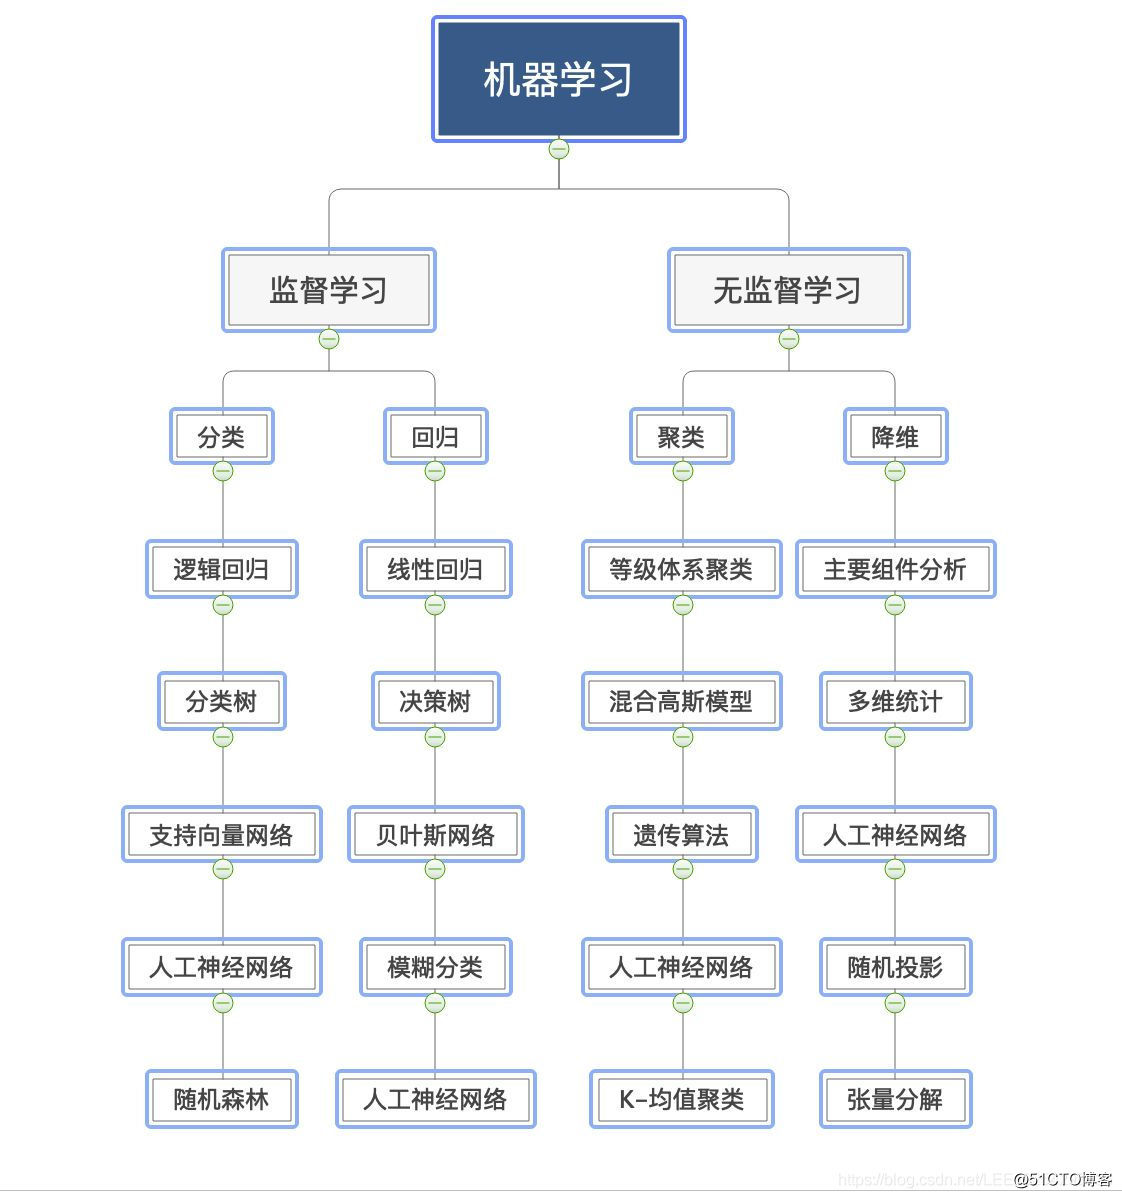
\includegraphics[width=.9\textwidth]{../lib/机器学习.jpeg}
        \column{0.35\linewidth}
        机器学习深究的话,需要学习很多数学和计算机知识。
        但是工业界将常用的机器学习算法封装地很好(如pytorch, scikit-learn),几行代码就可以实现一个模型。

        本文主要参考了\textcite{scikit-learn}的文档,在编码过程中阅读文档是有帮助的。
    \end{columns}
\end{frame}
% \subsection{一点建议}
% \begin{frame}
%     \frametitle{要学习机器学习吗?}
%     \begin{itemize}
%         \item 了解一下常见算法的思想和适用场景
%         \item 学好专业课和数学
%         \item 有问题查文档
%     \end{itemize}
% \end{frame}
\section{机器学习预测信用评级}
\subsection{数据预处理}
\begin{frame}
    \frametitle{数据来源}
    数据来自 \href{https://www.kaggle.com/datasets/agewerc/corporate-credit-rating}{kaggle}。
    涵盖了 2029 家美国上市公司信用评级的历史数据。数据除了公司基本信息外,还包括了30个财务特征:

    \begin{enumerate}
        \item 流动性指标: currentRatio, quickRatio, cashRatio, daysOfSalesOutstanding
        \item 盈利能力: grossProfitMargin, operatingProfitMargin, pretaxProfitMargin, netProfitMargin, effectiveTaxRate, returnOnAssets, returnOnEquity, returnOnCapitalEmployed
        \item 负债比率: debtRatio, debtEquityRatio
        \item 营运表现: assetTurnover, fixedasset
        \item 现金流指标: operatingCashFlowPerShare, freeCashFlowPerShare, cashPerShare, operatingCashFlowSalesRatio, freeCashFlowOperatingCashFlowRatio
    \end{enumerate}
\end{frame}
\begin{frame}[fragile]
    \frametitle{数据简单处理}
    评级分布如图\ref{rating}所示。
    我们会合并 C/CC/CCC 的评级,选取 3/4 作为训练集,1/4 作为测试集。
    \begin{figure}
        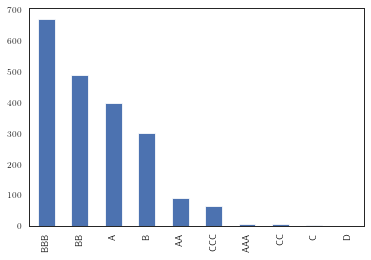
\includegraphics[width=0.6\linewidth]{../lib/rating.png}
        \label{rating}
        \caption{评级分布}
    \end{figure}
\end{frame}
\begin{frame}[fragile]
    \frametitle{数据简单处理}
    \begin{minted}{python}
import pandas as pd
import matplotlib.pyplot as plt
import seaborn as sns
df = pd.read_csv("./corporate_rating.csv", encoding="utf-8")
Y = df["Rating"].replace({"CCC": "C", "CC": "C"})
df["Date"] = df["Date"].apply(lambda x: x.split("/")[-1])
dummies = ["Rating Agency Name", "Sector", "Date"]
X = df[[i for i in df.columns if df[i].dtype != "object"]]
X = pd.concat([X]+[pd.get_dummies(df[i], drop_first=True)
    for i in dummies]),
    axis=1)
Xtrain, Xtest, Ytrain, Ytest = train_test_split(
    X, Y, test_size=0.25, random_state=42
)
\end{minted}
\end{frame}
\begin{frame}
    \frametitle{评价机器学习效果的指标}
    对于二分类问题,一个样本真实情况可能是 True/False,对应预测可能是 Positive/Negative。
    \begin{center}
        \begin{tabular}{lll}
                     & True & False \\
            Positive & TP   & FP    \\
            Negative & TN   & FN    \\
        \end{tabular}
    \end{center}
    准不准的定义有这么几种:
    \begin{eqnarray}
        precision & = & TP / (TP + FP) \\
        recall & = & TP / (TP + FN) \nonumber\\
        F1 & = & \frac{precision\cdot recall}{precision+recall}\nonumber
    \end{eqnarray}
    分别为 预测阳性中真实为正的概率、样本中的正例有多少被预测正确、以及二者的调和平均。
\end{frame}

\begin{frame}[fragile]
    \frametitle{评价机器学习效果的指标}
    除此之外,我们再来比较一下“相关系数”,看一看预测差异是否很大。
    \begin{minted}{python}
def get_score(Xtest, Ytrue, model):
    Ypred = model(Xtest)
    avg = "weighted"
    rating_map = {i: ord(i[0]) * 100 - len(i)
                    for i in Y.unique()}
    return {
        "precision":
            precision_score(Ytrue, Ypred, average=avg),
        "recall": recall_score(Ytrue, Ypred, average=avg),
        "f1": f1_score(Ytrue, Ypred, average=avg),
        "\(R^2\)": pearsonr(
            [rating_map[i] for i in Ypred],
            [rating_map[i] for i in Ytest]
        )[0],
    }
\end{minted}
\end{frame}
\begin{frame}
    \frametitle{完全随机的情况}
    如果我们训练的分类器完全无效,那么结果是
    \begin{center}
        \begin{tabular}{ll}
            precision & 0.2364 \\
            recall    & 0.1254 \\
            f1        & 0.1544 \\
            \(R^2\)   & 0.0089 \\
        \end{tabular}
    \end{center}
\end{frame}
\subsection{神经网络}
\subsubsection{多层感知机}
\begin{frame}
    \frametitle{Why Neural Networks can learn almost anything\footnote{\href{https://www.youtube.com/watch?v=0QczhVg5HaI}{youtube视频}}}
    函数是抽象现实世界的好方法,如 \(\displaystyle F=G\frac{Mm}{R^2}\),但是我们经常遇到的是并不知道函数的解析形式而只知道某几个点的值。

    神经网络是源于对生物神经的模拟,是一种通用的函数估计方法\cite{hornik1989multilayer},通过已知的点训练出神经网络 $f$ ,我们可以用它来预测未知的 $x$ 为 $f(x)$ ,尽管这个 $f$ 不一定是解析的。

    \begin{center}
        \href{https://playground.tensorflow.org/}{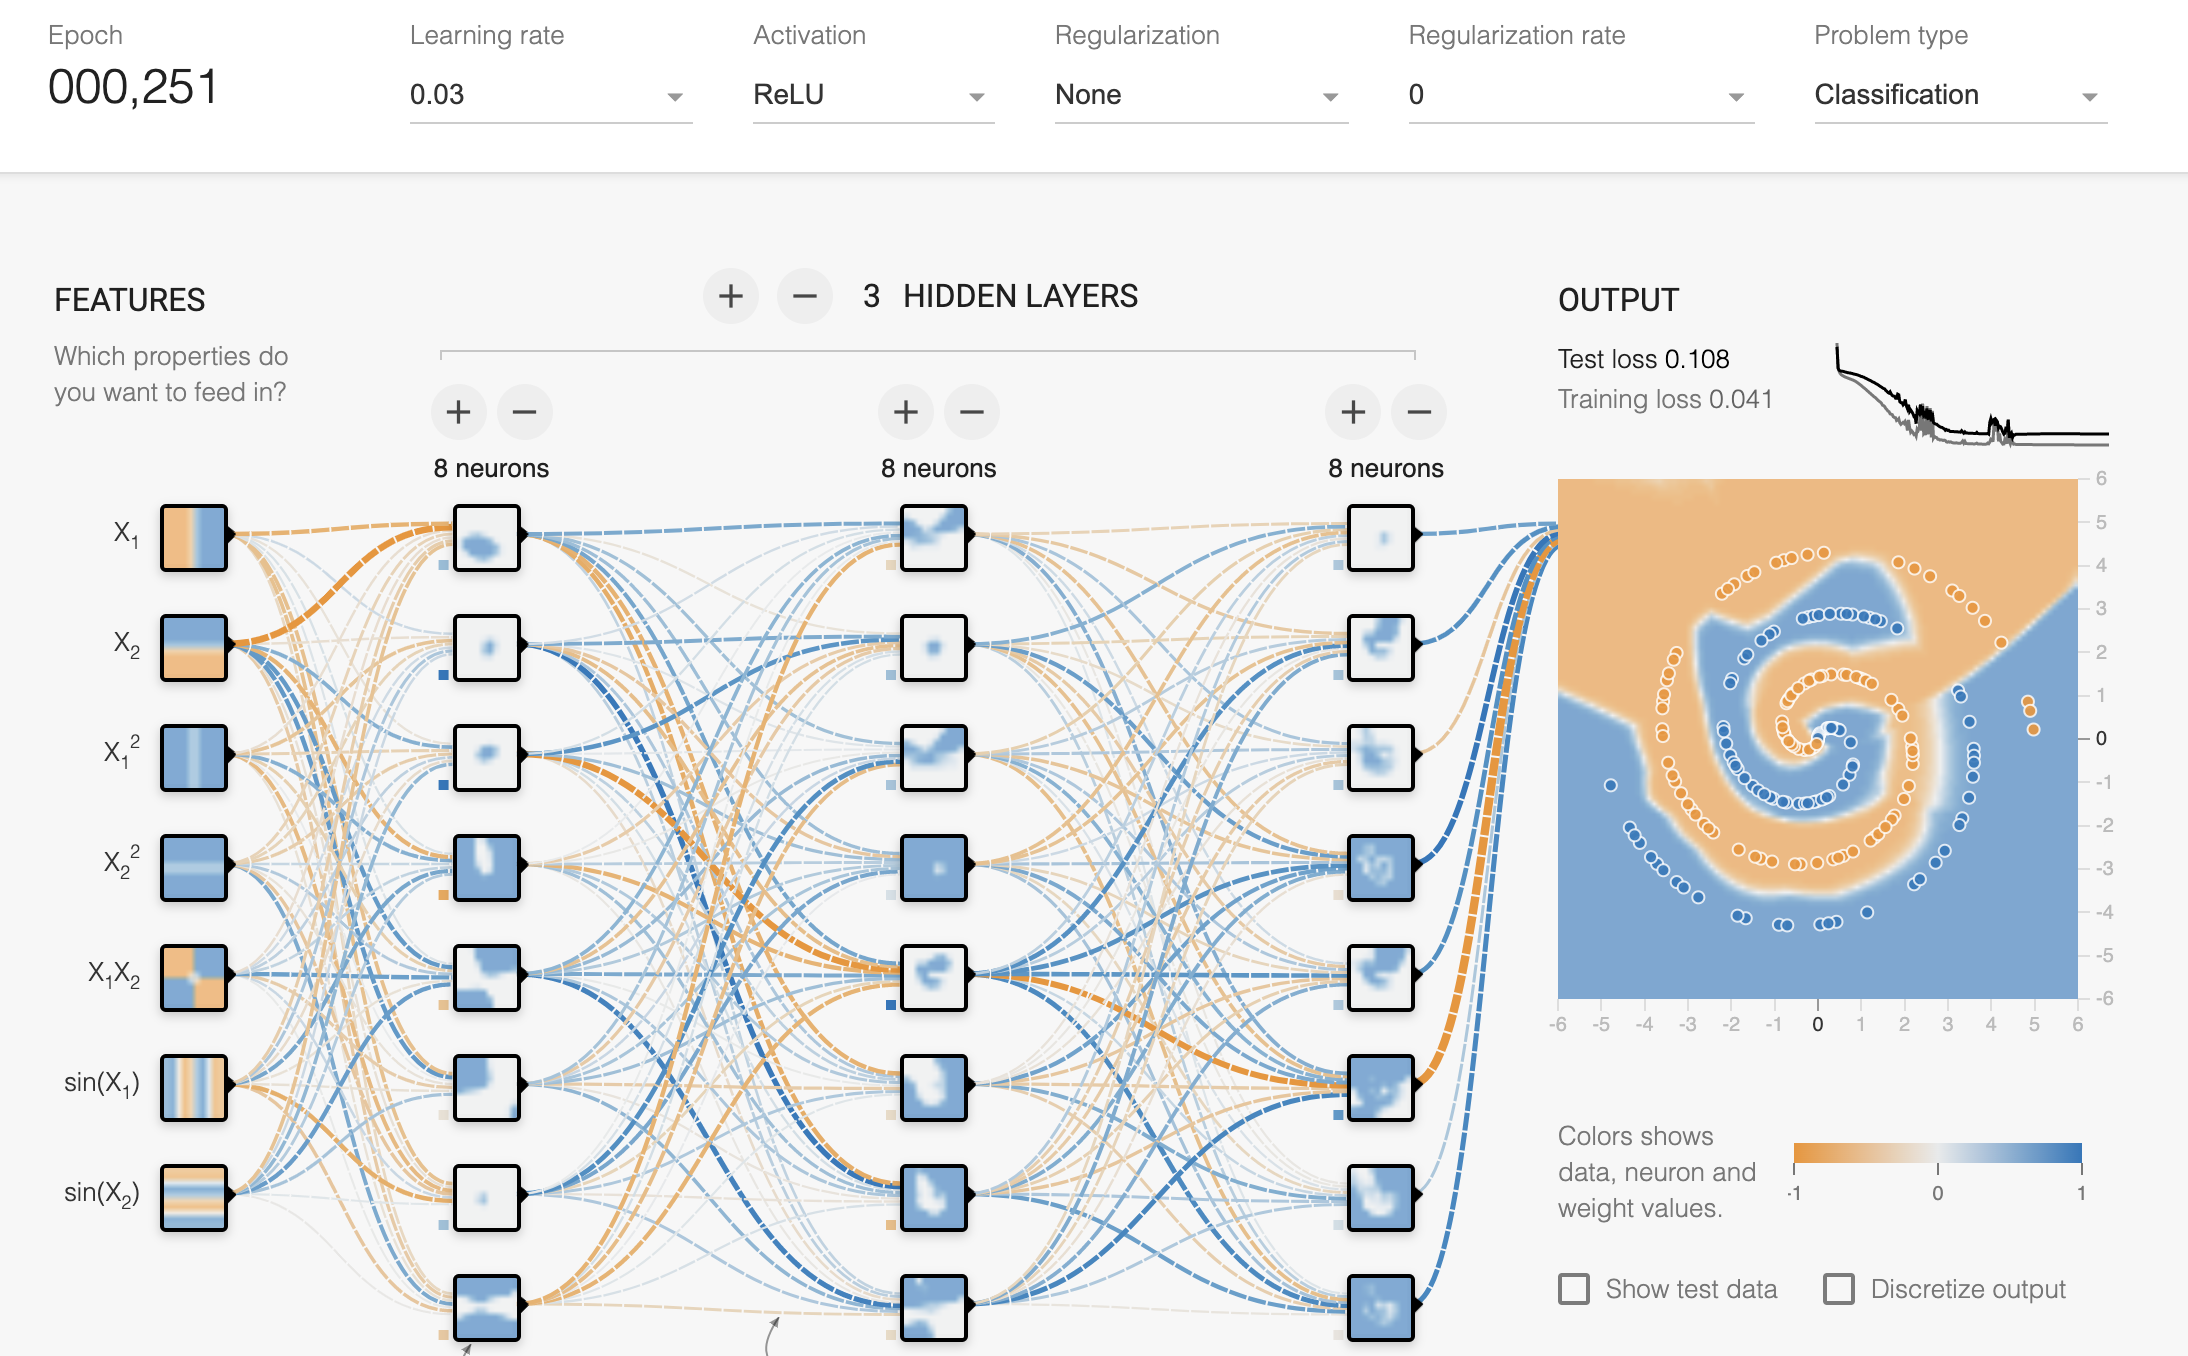
\includegraphics[width=0.7\linewidth]{../lib/tfplay.png}}
    \end{center}
\end{frame}

\begin{frame}
    \frametitle{梯度下降与反向传播}
    \begin{columns}
        \column{0.5\linewidth}
        \begin{figure}
            \centering
            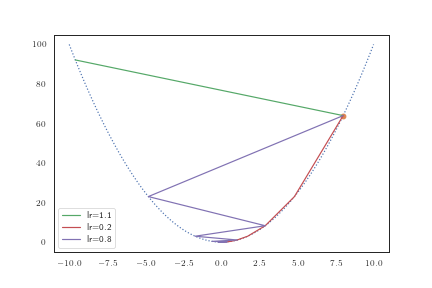
\includegraphics[width=\linewidth]{../lib/lr.png}
            \caption{不同学习率的影响}
        \end{figure}
        \column{0.5\linewidth}
        先看最简单的线性的情况。假设有一个我们不知道 $w,b$ 的线性的 $y=wx+b$ ,仅知道若干个 $(x,y)$。

        首先定义 \textbf{损失函数} 为 $loss = \sum{(\hat{y}-y)^2}$ ,即 $loss(w, b)=\sum(wx+b-y)^2$ 。我们要最小化估计的损失函数。

        令 $w=w_0,b=b_0$ ,正向计算得到 $loss(w_0,b_0)$。
        为了最小化它,我们让 $w,b$ 沿着 $loss$ 的梯度走一小步(\textbf{learning rate}),即误差反向传播。
        不断迭代,逼近 $loss(w,b)$ 的最小值,得到估计的 $w^*,b^*$。
    \end{columns}
\end{frame}

\begin{frame}[fragile]
    \frametitle{梯度下降与反向传播}
    左边的代码是我们手动实现的上述过程,右边的代码是更加 pytorch 风格的代码。
    \begin{columns}
        \column{0.5\linewidth}
        \tiny\begin{minted}{python}
import torch 
x = torch.rand([500,1]) # 张量可以当成是特殊的向量
y_true = 3*x+8
learning_rate = 0.05 
# w b 自动求导
w = torch.tensor([[0]], requires_grad=True) 
b = torch.tensor(0, requires_grad=True
                    , dtype=torch.float32)
for i in range(500):
    y_pred = torch.matmul(x,w)+b # 预测值
    loss = (y_true-y_pred).pow(2).mean() # loss(w, b)
    if w.grad is not None: # 不清零会累加
        w.grad.data.zero_()
    if b.grad is not None:
        b.grad.data.zero_()
    loss.backward() # 反向传播得到梯度
    w.data = w.data - w.grad*learning_rate
    b.data = b.data - b.grad*learning_rate
    if i % 50 == 0:
        print(w.item(), b.item(), loss.item())
\end{minted}
        \column{0.5\linewidth}
        \tiny\begin{minted}{python}
import torch
from torch import nn,optim
class Lr(nn.Module):
    def __init__(self):
        super(Lr, self).__init__()
        self.layer = nn.Linear(1,1)
    def forward(self, x):
        return self.layer(x)
x = torch.rand([500,1])
y = 3*x+8
model = Lr()
criterion = nn.MSELoss()
optimizer = optim.SGD(model.parameters(), lr=0.05)
for i in range(500):
    out = model(x)
    loss = criterion(y, out)
    optimizer.zero_grad()
    loss.backward()
    optimizer.step()
list(model.parameters())
        \end{minted}
    \end{columns}
\end{frame}
\begin{frame}
    \frametitle{激活函数}
    \begin{columns}
        \column{0.5\linewidth}
        \begin{figure}
            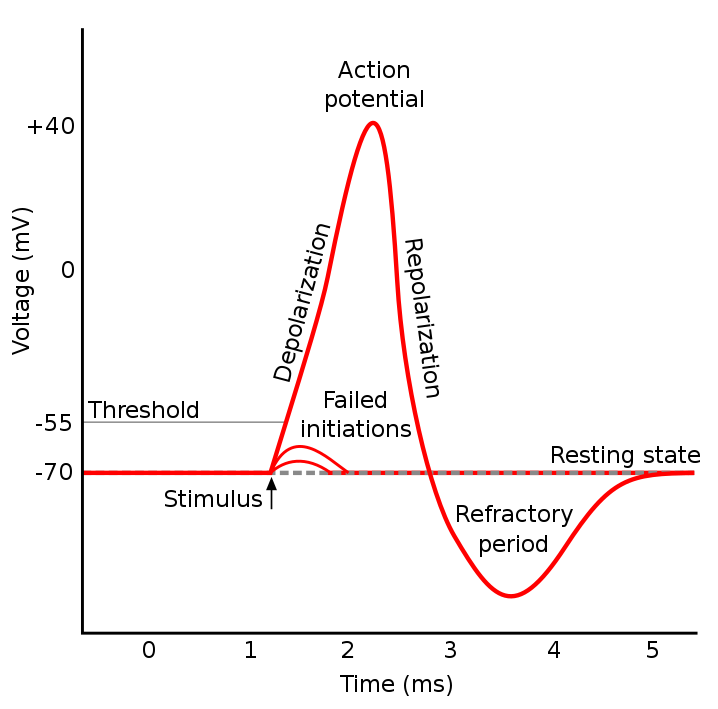
\includegraphics[width=\linewidth]{../lib/neuron.png}
            \caption{生物神经的动作电位}            
        \end{figure}

        \column{0.5\linewidth}
        线性函数的叠加仍然是线性函数。为了实现对非线形特征的识别,也为了对生物神经有更好的模拟,神经网络中每个神经元的输入添加了非线性的“\textbf{激活函数}”。常见的有:

        \begin{eqnarray}
            ReLU(x)&=&\max(0,x)\\
            Sigmoid(x)&=&\frac {1}{1+e^{-x}}\\
            tanh(x)&=&\tanh{x}\\
            Softmax(x_i)&=&\frac{e^{x_i}}{\sum e^{x_j}}
        \end{eqnarray}

    \end{columns}
\end{frame}

\begin{frame}[fragile]
    \frametitle{神经网络}
    一层神经元的输出,作为另一层神经网络的输入,就形成了一层神经网络。多层神经网络通过损失函数和优化器迭代训练,就形成了一个简单的感知机。

    \begin{columns}
        \column{0.7\linewidth}
        \tiny\begin{minted}{python}
from torch import nn
import torch
Ytrain_nn = torch.tensor(pd.get_dummies(Ytrain).values, 
                dtype=torch.float32)
Xtrain_nn = torch.tensor(Xtrain.values, dtype=torch.float32)
net = nn.Sequential(
    nn.Linear(Xtrain_nn.shape[1], 40),
    nn.ReLU(),
    nn.Linear(40, 7),
    nn.Softmax(dim=1)
)
optimizer = torch.optim.SGD(net.parameters(), lr=0.001)
loss_func = torch.nn.MSELoss()
for t in range(10000):
    prediction = net(Xtrain_nn)
    loss = loss_func(Ytrain_nn, prediction)
    optimizer.zero_grad()
    loss.backward()
    optimizer.step()
Xtest_nn = torch.tensor(Xtest.values, dtype=torch.float32)
prediction = pd.DataFrame(net(Xtest_nn).detach().numpy())           
        \end{minted}
        \column{0.3\linewidth}
        \begin{tabular}{ll}
            precision & 0.2739  \\
            recall    & 0.3386  \\
            f1        & 0.2763  \\
            \(R^2\)   & -0.059 \\
        \end{tabular}
    \end{columns}
\end{frame}
\subsubsection{CNN}
\begin{frame}
    \frametitle{卷积}
\end{frame}
\begin{frame}
    \frametitle{实现 CNN}
\end{frame}
\subsubsection{RNN}
\begin{frame}
    \frametitle{“记忆”}
\end{frame}
\begin{frame}
    \frametitle{实现 LSTM}
\end{frame}
\begin{frame}
    \frametitle{其他神经网络}
\end{frame}
\subsection{经典机器学习算法}
\subsubsection{从logit模型开始}
\begin{frame}[fragile]
    \frametitle{logit 模型}
    关于分类我们自然地想到了 logit 回归。我们不妨以 logit 回归为切入点看一看 sklearn 是如何训练模型的:

    \begin{minted}{python}
from sklearn.linear_model import LogisticRegression
logit = LogisticRegression(solver="saga", 
            multi_class="multinomial", random_state=42)
logit.fit(Xtrain, Ytrain)
logit.predict(Xtest)
    \end{minted}

    \begin{center}
        \begin{tabular}{ll}
            precision & 0.1815  \\
            recall    & 0.2440  \\
            f1        & 0.1547  \\
            \(R^2\)   & -0.0177 \\
        \end{tabular}
    \end{center}
\end{frame}
\subsubsection{基于树的算法}
\begin{frame}[fragile]
    \frametitle{决策树}

    决策树直观上很好理解,也是我们今天少数可解释的模型。一个数据集有多个特征,每个节点按照某个特征是否满足一定的条件分叉,形成一棵二叉树。

    该节点选取特征分叉的决策依据是最大化“信息增益”,即分叉前后数据更“有序”,且更有序的程度最大(信息熵变化最大)。
    这棵树为了避免过拟合,我们会对决策树“剪枝”,增加一些分支条件的限制,可以看\href{https://scikit-learn.org/stable/modules/generated/sklearn.tree.DecisionTreeClassifier.html}{sklearn 文档}。
    \begin{center}
        \begin{figure}
            \includegraphics[width=0.8\linewidth]{/Users/dcy/Desktop/thesis/data/decision_tree.png}
            \label{decisiontree}
            \caption{决策树}
        \end{figure}
    \end{center}
\end{frame}
\begin{frame}
    \frametitle{集成学习}
    决策树一般是一种比较弱的分类器。集成学习则是利用多个弱分类器的集成,形成一个强分类器。

    组合的方法常见的有两种:bagging 和 boosting。bagging 是平行地训练弱分类器然后投票,特点是不容易过拟合。
    典型的随机森林就是随机地选取样本和特征训练出一棵棵决策树后投票,如图 \ref{randomforest} 所示。
    \begin{center}
        \begin{figure}
            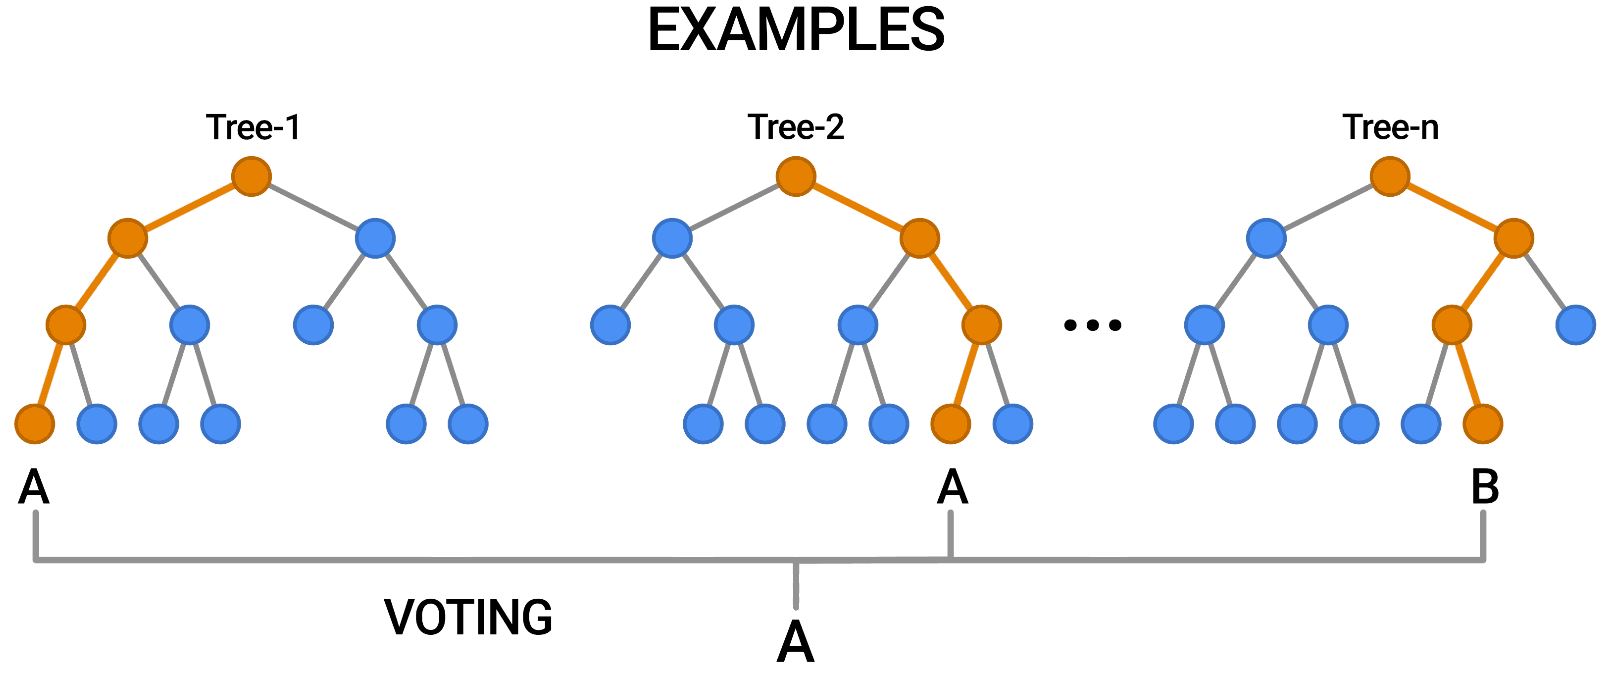
\includegraphics[width=0.8\linewidth]{../lib/rf.png}
            \label{randomforest}
            \caption{随机森林}
        \end{figure}
    \end{center}

\end{frame}
\begin{frame}
    \frametitle{集成学习}
    使用 boosting 的梯度提升树可以树的深度很少就能达到很高的精度。
    boosting 迭代地训练一系列的分类器,每个分类器采用的样本分布都和上一轮的学习结果有关,直观比方是每个树都去学习上一个树没有学习好的地方。
    \begin{center}
        \begin{figure}
            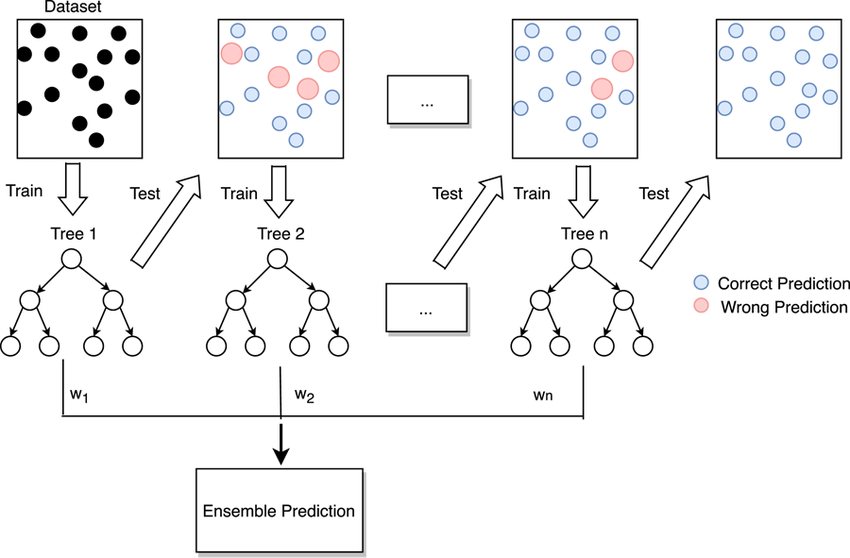
\includegraphics[width=0.6\linewidth]{../lib/boosting.png}
            \label{boosting}
            \caption{梯度提升树}
        \end{figure}
    \end{center}
\end{frame}
\begin{frame}[fragile]
    \frametitle{基于树的算法代码}
    \begin{minted}{python}
from sklearn.tree import DecisionTreeClassifier
from sklearn.ensemble import RandomForestClassifier
from sklearn.ensemble import GradientBoostingClassifier
dt = DecisionTreeClassifier(max_depth=3, random_state=42)
dt.fit(Xtrain, Ytrain)
rf = RandomForestClassifier(max_depth=4, random_state=42)
rf.fit(Xtrain, Ytrain)
gb = GradientBoostingClassifier(max_depth=3, random_state=42)
gb.fit(Xtrain, Ytrain)
    \end{minted}
    \begin{center}
        \begin{tabular}{l|cccc}
            model & precision & recall & f1     & \(R^2\) \\ \hline
            决策树   & 0.3498    & 0.3799 & 0.3529 & 0.3632  \\
            随机森林  & 0.3960    & 0.4251 & 0.3835 & 0.3995  \\
            梯度提升树 & 0.5305    & 0.5256 & 0.5095 & 0.5421  \\
        \end{tabular}
    \end{center}
\end{frame}
\subsubsection{基于距离的算法}
\begin{frame}
    \frametitle{支持向量机}
    SVM 的思想是样本分布在空间中,找到一个可以恰好划分开样本点、并且间隔最大的的(超)平面。

    当然这样的超平面不一定好找,我们可以用加入惩罚项的“软间隔”优化或者利用“核函数”将空间映射为可分的。

    \begin{center}
        \begin{figure}
            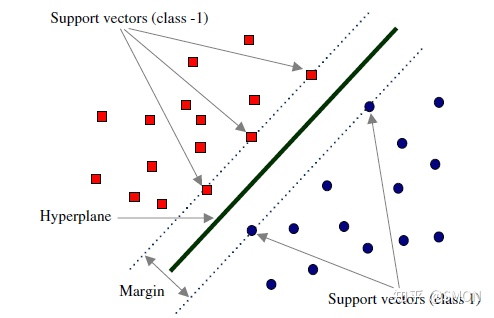
\includegraphics[width=0.6\linewidth]{../lib/SVM.jpeg}
            \caption{Support Vector Machine}
        \end{figure}
    \end{center}
\end{frame}
\begin{frame}
    \frametitle{KNN 与 K Means}
    \begin{columns}
        \column{0.5\linewidth}
        KNN 的思想是一个样本归属的分类属于离他最近的 K 个已经打好标签的邻居中占多数的分类,也非常直观。
        \column{0.5\linewidth}
        K Means 则是一种聚类算法,不需要打好标签(即所谓“无监督学习”),目的是把样本点归为 K 个群落。
        其思想是假设 K 个重心,样本根据与不同重心的距离归类,进而得到新的重心。
        以此循环往复,直至重心稳定下来。
    \end{columns}
\end{frame}
\begin{frame}[fragile]
    \frametitle{基于距离的算法实现}
    \begin{minted}{python}
from sklearn.neighbors import KNeighborsClassifier
from sklearn.svm import SVC

svm = SVC(kernel="rbf", gamma="auto", random_state=42)
svm.fit(Xtrain, Ytrain)
KNN = KNeighborsClassifier(n_neighbors=3)
KNN.fit(Xtrain, Ytrain)
    \end{minted}
    \begin{center}
        \begin{tabular}{l|cccc}
            model & precision & recall & f1     & \(R^2\) \\ \hline
            SVM   & 0.4137    & 0.4094 & 0.3517 & 0.3431  \\
            KNN   & 0.3625    & 0.3523 & 0.3420 & 0.2987  \\
        \end{tabular}
    \end{center}
\end{frame}
\subsection{对比}
\begin{frame}
    \frametitle{结果对比}
\end{frame}
\section{机器学习在企业风险管理中的应用}

\begin{frame}
    \frametitle{机器学习在企业风险管理中的应用}
    \Textcite{mai2019deep} 利用 CNN 预测企业破产,在处理文本数据时利用 word embedding 量化,AUC 曲线如图
    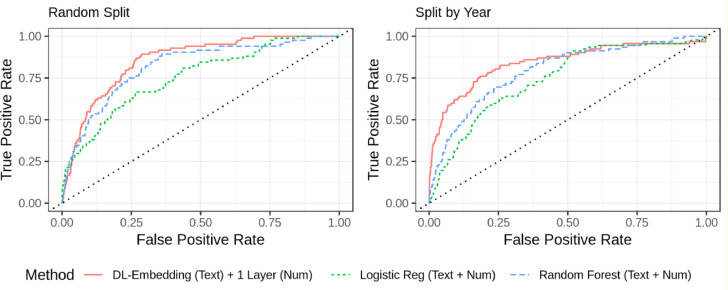
\includegraphics[width=\linewidth]{../lib/mlinerm.jpg}
\end{frame}
\begin{frame}
    \frametitle{机器学习在企业风险管理中的应用}
    \Textcite{kellner2022opening} 利用神经网络预测违约损失 Loss Given Default。

    他们将传统的分位数回归的回归元作为第一层,通过神经网络揭示其中的非线性关系,比如交叉项及其他非线性关系,神经网络最后一层是传统的分位数回归。利用 first order feature importance,量化输入变量的整体重要性。同时排除掉二阶的和交互的在分位数中接近于零。因此 QRNN 和分位数 QR 的分位数损失非常相似
    通过允许分位数回归神经网络实现的分位数中的非线性和相互作用来扩展这种方法。这种方法大大增强了建模的灵活性。额外的灵活性在更好地分布拟合和超时样本方面带来了回报,分位数预测精度提高了 30\%,同时更加 robust 。
\end{frame}
\begin{frame}
    \frametitle{机器学习在企业风险管理中的应用}
    \Textcite{golbayani2020comparative}
    使用决策树、随机森林、支持向量机和多层感知器应用于相同的数据集,预测公司未来评级。他们统计了机器学习在债券评级和公司信用评级方面的文章,很多认为 SVM 和神经网络是比较准确的。但是他们使用 Notches Distance 来对机器学习绩效来打分,认为基于决策树的两种方法更有效。

    当前机器学习最火热的两个应用方向是计算机视觉 CV 和自然语言处理 NLP ,亦有一些文献利用自然语言处理分析文本数据做研究。
\end{frame}

% 				这是我用两层神经网络的代码
% 				\begin{verbatim}

% result["bp neural network"] = get_score(Xtest, Ytest, lambda _: Ypredict)
% result["bp neural network"]
% \end{verbatim}
% 			\end{block}
% 		\end{block}

% 		\begin{block}{CNN}
% 			所谓卷积神经网络,就是用卷积核扫描,类似“锐化”,是一种比较经典的计算机视觉算法。图片之间的像素是有关系的,刚刚的神经网络显然没有考虑到连续像素的关联性,CNN 通过做卷积将关系呈现出来。
% 			\begin{center}
% 				\includegraphics[width=.9\linewidth]{/Users/dcy/.emacs.d/.local/cache/org-persist/da/21d33e-ccf0-49f3-8b8f-bd424c5d6978-011bffe9337373ece605a2705d648ce1.jpg}
% 			\end{center}

% 			\href{https://zh.m.wikipedia.org/zh-hans/\%E5\%8D\%B7\%E7\%A7\%AF}{卷积}有其数学定义 \((f*g)(n) = \int_{-\infty}^{\infty}f(\tau)g(n-\tau)\mathrm{d}\tau\),简单地理解就是两个函数 \texttt{f} 和 \texttt{g} ,先对g函数进行翻转,相当于在数轴上把 \texttt{g} 函数从右边“卷”到左边去。然后再把 \texttt{g} 函数平移到 \texttt{n} ,在这个位置对两个函数的对应点相乘,然后相加(“积”)。

% 			卷积神经网络先用卷积层扫描出特征,然后利用“池化”增强稳健性防止过拟合,最后一个全连接层处理输出。图像可以由二维的位置和第三维(颜色 RGB )确定,在 \texttt{pytorch} 中常用 \texttt{Conv2d} 。而我们的数据则是一条条的,望文生义应该用 \texttt{Conv1d} (其实会用在自然语言处理中,但 RNN 应用更多)。

% 			从这里开始利用 CPU 训练比较慢,有 NVIDIA GPU 的同学可以尝试在 GPU 上训练
% 			\begin{verbatim}
% class CNN(nn.Module):
%     def __init__(self) -> None:
%         super(CNN, self).__init__()
%         self.conv = nn.Sequential(
%             nn.Conv1d(Xtrain_nn.shape[1], 20, 3, padding=3),
%             nn.Tanh(),
%             nn.AvgPool1d(2),
%         )
%         self.fc = nn.Sequential(
%             nn.Linear(40, len(encode)),
%             nn.ReLU(),
%             nn.Softmax(dim=1),
%         )

%     def forward(self, x):
%         out = self.conv(x)
%         out = out.view(out.size(0), -1)
%         out = self.fc(out)
%         return out
% Xtrain_cnn = Xtrain_nn.unsqueeze(2)
% Xtest_cnn = Xtest_nn.unsqueeze(2)
% net = CNN()
% optimizer = torch.optim.Adamax(net.parameters())
% loss_func = torch.nn.L1Loss()
% epochnum = 10000
% for epoch in range(epochnum):
%     prediction = net(Xtrain_cnn)
%     loss = loss_func(Ytrain_nn, prediction)
%     optimizer.zero_grad()
%     loss.backward()
%     optimizer.step()
%     if epoch % (epochnum / 10) == 0:
%         print("epoch:", epoch, "loss:", loss.item())
% prediction = pd.DataFrame(net(Xtest_cnn).detach().numpy())
% Ypredict = prediction.idxmax(axis=1).map(lambda x: encode[x])
% result["CNN"] = get_score(Xtest, Ytest, lambda _: Ypredict)
% result["CNN"]
% \end{verbatim}

% 			增加网络层数可能会导致梯度离散和梯度爆炸的情况,反而效果不好。残差网络 ResNet 利用在网络间加入 shortcut ,使更深层次的训练结果至少不差于更浅层次(如果更差就直接走 shortcut )
% 		\end{block}
% 		\begin{block}{RNN}
% 			\begin{center}
% 				\includegraphics[width=.9\linewidth]{/Users/dcy/.emacs.d/.local/cache/org-persist/e7/a5e28e-ecf0-4f90-b7d8-77777a921d3d-0ae5bdb1bc5eed3623ce9cfa0b704d21.jpg}
% 			\end{center}
% 			循环神经网络:常用在 NLP 中并大放异彩,也会应用在股价等时间序列中。他会短期地“记住”参数,就如同我说这句话的时候你短期地记住了上一句话,会更新“自我”而非直接向前传递,在该层中“循环”。即对于隐藏层而言,\(h_t = f_w(h_{t-1}, x_t)\) 。随着输入的更新,有一个短暂的 memory ,记住刚刚的参数。
% 			\begin{verbatim}

% class LSTM(nn.Module):
%     def __init__(self):
%         super(LSTM, self).__init__()
%         self.lstm = nn.LSTM(
%             input_size=1,
%             hidden_size=32,
%             num_layers=1,
%             batch_first=True,
%             bidirectional=True,
%         )
%         self.fc = nn.Linear(32* 2, num_classes)

%     def forward(self, x):
%         # x, _ = x
%         out, _ = self.lstm(x)
%         out = self.fc(out[:, -1, :])
%         return out


% input_size = 1
% hidden_size = 32
% num_layers = 1
% num_classes = 7
% net = LSTM()
% optimizer = torch.optim.Adamax(net.parameters())
% loss_func = nn.MSELoss()
% epochnum = 3000
% for epoch in range(epochnum):
%     out = net(Xtrain_nn.unsqueeze(2))
%     loss = loss_func(out, Ytrain_nn)
%     optimizer.zero_grad()
%     loss.backward()
%     optimizer.step()
%     if epoch % (epochnum / 10) == 0:
%         print("epoch:", epoch, "loss:", loss.item())

% prediction = pd.DataFrame(net(Xtest_nn.unsqueeze(2)).detach().numpy())
% Ypredict = prediction.idxmax(axis=1).map(lambda x: encode[x])
% result["RNN"] = get_score(Xtest, Ytest, lambda _: Ypredict)
% result["RNN"]
% \end{verbatim}

% 			但是 RNN 的的梯度非常容易“爆炸”(特别大)或“离散”(特别小以致于不更新),预测可能会出错。
% 			针对此,LSTM (Long Short Term Memory)模型设计了三个“门”:输入门 \texttt{i} ,遗忘门 \texttt{f} ,输出门 \texttt{o} ,有一篇非常好的\href{https://colah.github.io/posts/2015-08-Understanding-LSTMs/}{blog}详细描述了这些门是如何工作的,简而言之他加入了长期记忆的部分。
% 		\end{block}

% 		\begin{block}{GAN \& RL}
% 			\begin{itemize}
% 				\item 生成对抗网络:随机取样作为输入,其输出结果需要尽量模仿训练集中的真实样本,使判别网络无法判断生成网络的输出结果是否真实
% 				\item 强化学习:博弈论……
% 			\end{itemize}
% 			\begin{quote}
% 				强化学习(RL)是机器学习的一个领域,涉及软件代理如何在环境中采取行动以最大化一些累积奖励的概念。该问题由于其一般性,在许多其他学科中得到研究,如博弈论,控制理论,运筹学,信息论,基于仿真的优化,多智能体系统,群智能,统计和遗传算法。。在运筹学和控制文献中,强化学习被称为近似动态规划或神经动态规划。--Wikipedia
% 			\end{quote}
% 		\end{block}
% 	\end{block}

% 	\begin{block}{对比}
% 		\begin{verbatim}
% feature = ["precision", "recall", "f1", "\(R^2\)"]
% [["model"]+feature]+list([i[0]]+ [round(j,4) for j in i[1].values()] for i in result.items())
% \end{verbatim}

% 		\begin{verbatim}
% N = len(feature)
% angles = np.linspace(0, 2 * np.pi, N, endpoint=False)
% angles = np.concatenate((angles, [angles[0]]))
% fig = plt.figure()
% ax = fig.add_subplot(111, polar=True)
% for model in result:
%     values = [i for i in result[model].values()] + [result[model]["precision"]]
%     ax.plot(angles, values, label=model)
%     ax.fill(angles, values, alpha=0.1)
% ax.set_thetagrids(angles[:-1] * 180 / np.pi, feature)
% ax.grid(True)
% plt.legend(bbox_to_anchor=(1.2, -0.1), ncol=3)
% plt.show()
% \end{verbatim}
% 	\end{block}
% \end{frame}
\section{参考文献}
\begin{frame}{参考文献}
    \printbibliography
\end{frame}
\end{document}
